\begin{figure}[!htbp]
\caption{Distribution of District Group Shares}
\begin{centering}
%\centering
%\fbox{
  \begin{tabular}{@{}cc@{}}
	% & & \\  	
  	\small (A) Same-Party Share &
    \small (B) Non-Same-Party Share  \\
    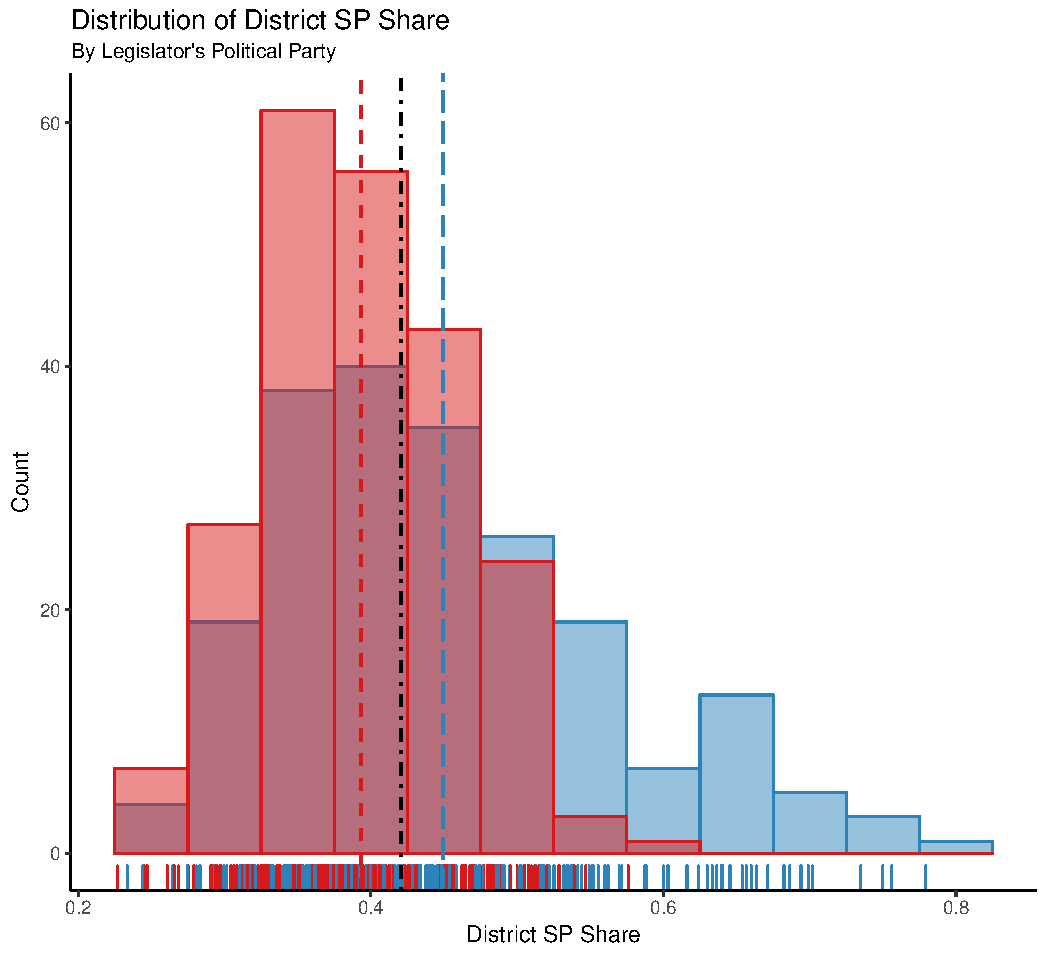
\includegraphics[width=.45\textwidth]{/Users/dsimp/GitHub/Clinton(2006)Rep/drafts/histogram/histogram2-1.pdf} &
    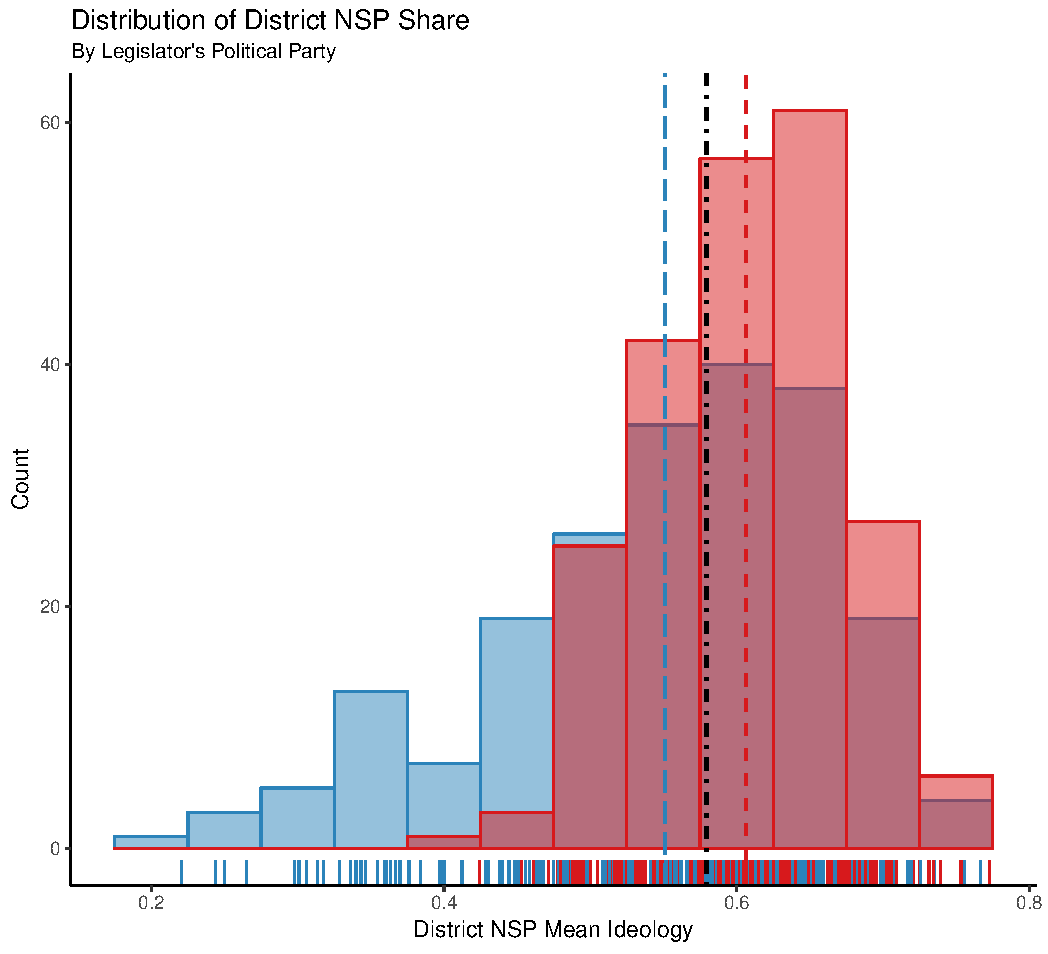
\includegraphics[width=.45\textwidth]{/Users/dsimp/GitHub/Clinton(2006)Rep/drafts/histogram/histogram2-2.pdf} \\
    % & & \\
    \small (C) Opposite-Party Share & 
    \small (D) Independent Share\\
    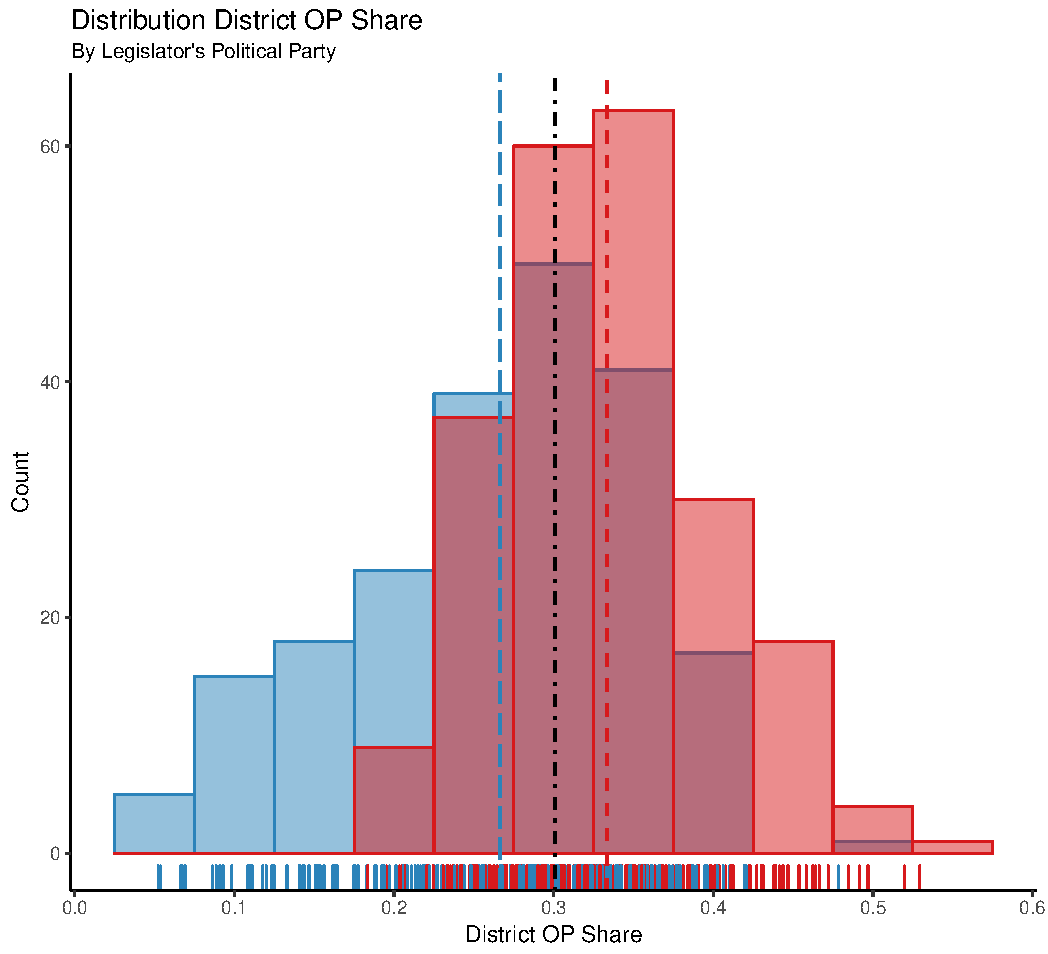
\includegraphics[width=.45\textwidth]{/Users/dsimp/GitHub/Clinton(2006)Rep/drafts/histogram/histogram2-3.pdf} &
    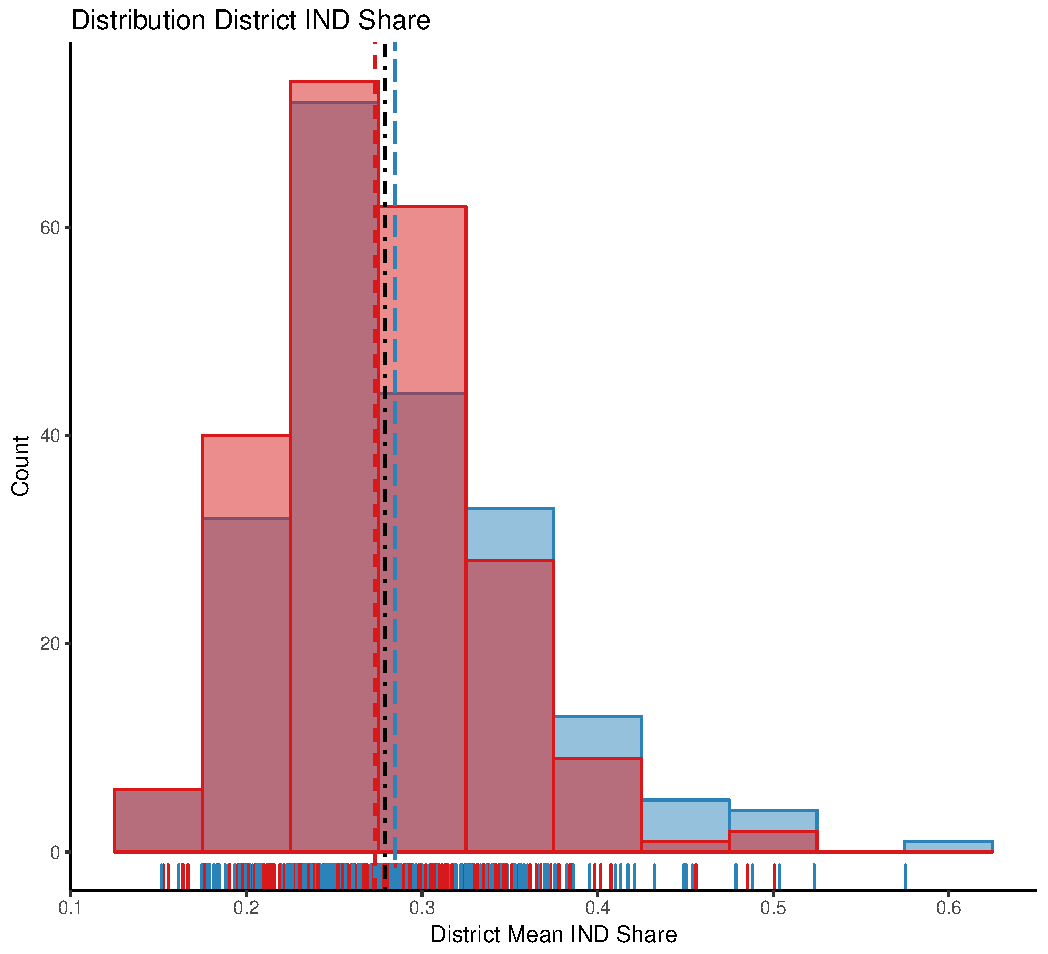
\includegraphics[width=.45\textwidth]{/Users/dsimp/GitHub/Clinton(2006)Rep/drafts/histogram/histogram2-4.pdf} \\
    % &  &\\
  \end{tabular}
    %}   
 \end{centering}
 \small~~~~~~~~\textbf{Note:} The histograms illustrate the distribution of constituency group share of total district voters. Districts are classified by the party of their legislator. The short dashed lines are the Republican controlled district means, the long dashed line are the Democratic controlled district means, and the dotted and dashed line is the chamber mean.
\end{figure}.